\documentclass[tikz,border=5pt]{standalone}
\usepackage{pgfplots}
\pgfplotsset{compat=1.18}

\definecolor{corba}{HTML}{365FB3}
\definecolor{referencia}{HTML}{6B7280}

\begin{document}
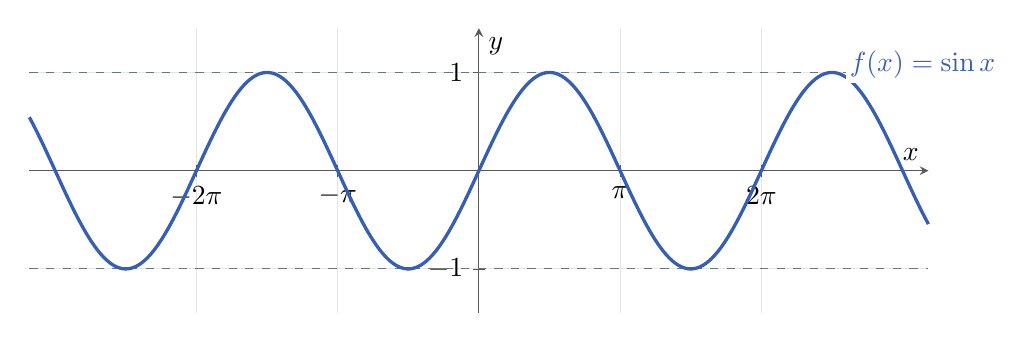
\begin{tikzpicture}
  \begin{axis}[
    width=13cm,
    height=5.2cm,
    axis lines=middle,
    xmin=-10,
    xmax=10,
    ymin=-1.45,
    ymax=1.45,
    xlabel={$x$},
    ylabel={$y$},
    xtick={-6.2832,-3.1416,0,3.1416,6.2832},
    xticklabels={$-2\pi$,$-\pi$,$0$,$\pi$,$2\pi$},
    ytick={-1,1},
    axis line style={black!65},
    tick style={black!65},
    grid=major,
    grid style={black!10},
    clip=false,
  ]
    \addplot[referencia, dashed, domain=-10:10] {1};
    \addplot[referencia, dashed, domain=-10:10] {-1};
    \addplot[corba, very thick, domain=-10:10, samples=320] {sin(deg(x))};
    \node[corba, anchor=west, fill=white, inner sep=1.5pt]
      at (axis cs:8.15,1.08) {$f(x)=\sin x$};
  \end{axis}
\end{tikzpicture}
\end{document}
